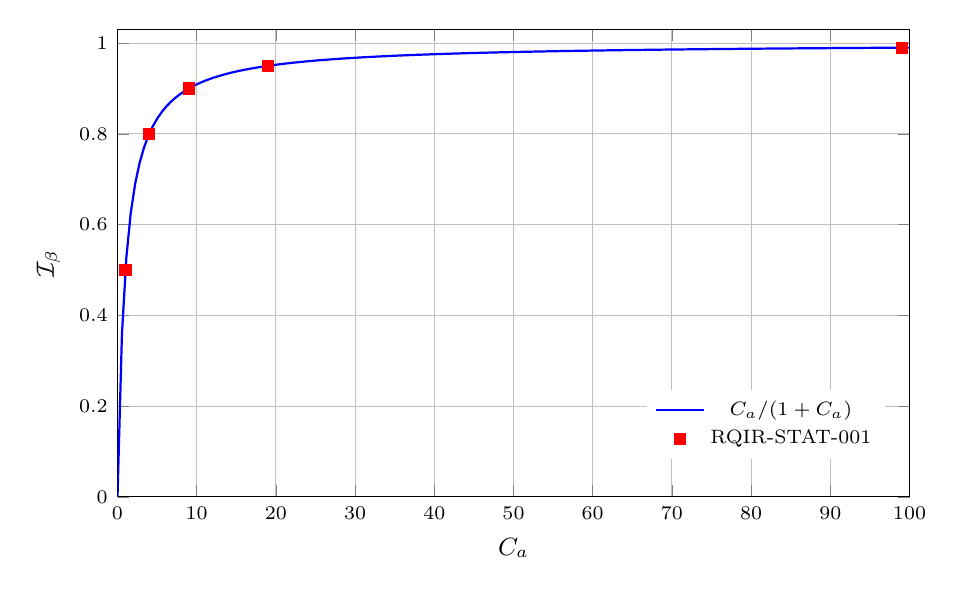
\begin{tikzpicture}
\begin{axis}[
 width=0.96\columnwidth,height=0.62\columnwidth,
 xlabel={$C_a$},ylabel={$\mathcal I_\beta$},
 xmin=0,xmax=100,ymin=0,ymax=1.03,
 grid=major,legend style={font=\scriptsize,draw=none,at={(0.97,0.08)},anchor=south east},
 tick label style={font=\scriptsize},label style={font=\small}]
\addplot[blue,thick,domain=0:100,samples=180] {x/(1+x)};
\addlegendentry{$C_a/(1+C_a)$}
\addplot[only marks,mark=square*,red] coordinates {(1,0.5) (4,0.8) (9,0.9) (19,0.95) (99,0.99)};
\addlegendentry{RQIR-STAT-001}
\end{axis}
\end{tikzpicture}
